\section{Probabilités et Dénombrement}

\subsection{Concepts fondamentaux}

\begin{intuitionbox}[Nécessité d'un Cadre Formel]
Avant de calculer des probabilités, il est crucial de définir les règles du jeu :
\newline
\textbf{Qu'est-ce qui peut arriver ?}
\newline
On définit l'ensemble de tous les résultats possibles de l'expérience.
\newline
\textbf{À quoi s'intéresse-t-on ?} 
\newline
On identifie les sous-ensembles de résultats spécifiques qui nous intéressent.
\newline
Ces deux idées nous conduisent aux notions d'Univers et d'Événement, qui sont les piliers de toute théorie des probabilités.
\end{intuitionbox}

\begin{definitionbox}[Concepts Fondamentaux]
\textbf{Univers (ou Espace Échantillon), $S$ :} 
\newline
L'ensemble de tous les résultats possibles d'une expérience aléatoire.
\newline
\textbf{Événement, $A$ :} 
\newline
Un sous-ensemble de l'univers ($A \subseteq S$). C'est un ensemble de résultats auxquels on s'intéresse.
\end{definitionbox}

\begin{examplebox}[Univers et Événement]
Pour l'expérience du "lancer d'un dé à six faces" :
\newline
L'\textbf{univers} est $S = \{1, 2, 3, 4, 5, 6\}$.
"Obtenir un nombre impair" est un événement, représenté par le sous-ensemble $A = \{1, 3, 5\}$.
\end{examplebox}

\subsection{Définition Naïve de la Probabilité}

\begin{definitionbox}[Probabilité Naïve]
Pour une expérience où chaque issue dans un espace échantillon fini $S$ est équiprobable, la probabilité d'un événement $A$ est le rapport du nombre d'issues favorables à $A$ sur le nombre total d'issues :
$$ P(A) = \frac{\text{Nombre d'issues favorables}}{\text{Nombre total d'issues}} = \frac{|A|}{|S|} $$
\end{definitionbox}

\begin{examplebox}[Applications de la définition naïve]
\begin{enumerate}
    \item \textbf{Lancer une pièce équilibrée :}
    L'espace échantillon est $S = \{\text{Pile, Face}\}$, donc $|S| = 2$.
    Si l'événement $A$ est "obtenir Pile", alors $A = \{\text{Pile}\}$ et $|A| = 1$.
    La probabilité est $P(A) = \frac{1}{2}$.

    \item \textbf{Lancer un dé à six faces non pipé :}
    L'espace échantillon est $S = \{1, 2, 3, 4, 5, 6\}$, donc $|S| = 6$.
    Si l'événement $B$ est "obtenir un nombre pair", alors $B = \{2, 4, 6\}$ et $|B| = 3$.
    La probabilité est $P(B) = \frac{3}{6} = \frac{1}{2}$.

    \item \textbf{Tirer une carte d'un jeu de 52 cartes :}
    L'espace échantillon $S$ contient 52 cartes, donc $|S| = 52$.
    Si l'événement $C$ est "tirer un Roi", il y a 4 Rois dans le jeu, donc $|C| = 4$.
    La probabilité est $P(C) = \frac{4}{52} = \frac{1}{13}$.
\end{enumerate}
\end{examplebox}

\subsection{Permutations (Arrangements)}

\begin{definitionbox}[Permutation de $k$ objets parmi $n$]
Le nombre de façons d'arranger $k$ objets choisis parmi $n$ objets distincts (où l'ordre compte et il n'y a pas de répétition) est noté $P(n, k)$ ou $A_n^k$ et est défini par :
$$ P(n, k) = \frac{n!}{(n-k)!} $$
où $n!$ est la factorielle de $n$, et par convention $0! = 1$.
\end{definitionbox}

\begin{intuitionbox}[Permutations de $k$ parmi $n$]
Pour placer $k$ objets dans un ordre spécifique en les choisissant parmi $n$ objets disponibles, on a $n$ choix pour la première position, $(n-1)$ choix pour la deuxième, ..., et $(n-k+1)$ choix pour la $k$-ième position. Cela donne $n \times (n-1) \times \cdots \times (n-k+1)$ arrangements. Ce produit contient $k$ termes. Il est égal à $\frac{n!}{(n-k)!}$, car cela revient à diviser la suite complète $n!$ par les facteurs non utilisés $(n-k) \times (n-k-1) \times \cdots \times 1$.
\end{intuitionbox}

\begin{examplebox}[Permutations de $k$ parmi $n$]
\textbf{Podium d'une course :} Une course réunit 8 coureurs. Combien y a-t-il de podiums (1er, 2e, 3e) possibles ? \\
On cherche le nombre de façons d'ordonner 3 coureurs parmi 8 : $P(8, 3)$. 
$$ P(8, 3) = \frac{8!}{(8-3)!} = \frac{8!}{5!} = 8 \times 7 \times 6 = 336 $$
Il y a 336 podiums possibles.
\end{examplebox}

\subsection{Le Coefficient Binomial}

\begin{theorembox}[Formule du Coefficient Binomial]
Le nombre de façons de choisir $k$ objets parmi un ensemble de $n$ objets distincts (sans remise et sans ordre) est donné par le coefficient binomial :
$$ \binom{n}{k} = \frac{n!}{k!(n-k)!} $$
\end{theorembox}

\begin{intuitionbox}

L’idée est de relier $\binom{n}{k}$ à quelque chose de plus facile à compter : les \textbf{permutations} de $k$ objets parmi $n$, c’est-à-dire les listes ordonnées.  
On sait qu’il y en a :
\[
P(n,k) = \frac{n!}{(n-k)!}.
\]

D’un autre côté, on peut construire chaque permutation en deux étapes :
\begin{enumerate}
    \item Choisir un \textbf{sous-ensemble} de $k$ objets (sans ordre), il y a $\binom{n}{k}$ façons de le faire.
    \item Ordonner ces $k$ objets, il y a $k!$ façons de le faire.
\end{enumerate}
Donc, le nombre total de permutations est aussi $\binom{n}{k} \cdot k!$.

\medskip

\noindent En égalisant les deux expressions :
\[
\binom{n}{k} \cdot k! = \frac{n!}{(n-k)!}
\quad\Longrightarrow\quad
\binom{n}{k} = \frac{n!}{k!(n-k)!}.
\]

\medskip

\noindent Pour rendre cela concret, voici le cas $\binom{5}{3}$.  
Il y a 10 sous-ensembles de 3 éléments parmi $\{a,b,c,d,e\}$. Chacun donne lieu à $3! = 6$ permutations.  
Le tableau ci-dessous montre \textbf{toutes les 60 permutations}, regroupées par sous-ensemble :

\begin{center}
\small
\renewcommand{\arraystretch}{0.9}
\setlength{\tabcolsep}{2pt}
\begin{tabular}{|c|c|c|c|c|c|c|c|c|c|}
\hline
\textbf{$\{a,b,c\}$} & \textbf{$\{a,b,d\}$} & \textbf{$\{a,b,e\}$} & \textbf{$\{a,c,d\}$} & \textbf{$\{a,c,e\}$} & \textbf{$\{a,d,e\}$} & \textbf{$\{b,c,d\}$} & \textbf{$\{b,c,e\}$} & \textbf{$\{b,d,e\}$} & \textbf{$\{c,d,e\}$} \\
\hline
$abc$ & $abd$ & $abe$ & $acd$ & $ace$ & $ade$ & $bcd$ & $bce$ & $bde$ & $cde$ \\
\hline
$acb$ & $adb$ & $aeb$ & $adc$ & $aec$ & $aed$ & $bdc$ & $bec$ & $bed$ & $ced$ \\
\hline
$bac$ & $bad$ & $bae$ & $cad$ & $cae$ & $dae$ & $cbd$ & $ceb$ & $dbe$ & $dce$ \\
\hline
$bca$ & $bda$ & $bea$ & $cda$ & $cea$ & $dea$ & $cdb$ & $ceb$ & $deb$ & $dec$ \\
\hline
$cab$ & $dab$ & $eab$ & $dac$ & $eac$ & $ead$ & $dbc$ & $ebc$ & $edb$ & $ecd$ \\
\hline
$cba$ & $dba$ & $eba$ & $dca$ & $eca$ & $eda$ & $dcb$ & $ebc$ & $edb$ & $edc$ \\
\hline
\end{tabular}
\end{center}

\smallskip

Chaque colonne correspond à \textbf{un seul et même choix non ordonné} (par exemple $\{a,b,c\}$), mais à 6 listes différentes selon l’ordre.  
Ainsi, pour obtenir le nombre de \textit{choix non ordonnés}, on divise le nombre total de listes ($60$) par le nombre d’ordres par groupe ($6$) :
\[
\binom{5}{3} = \frac{60}{6} = 10.
\]

\medskip

\noindent C’est exactement ce que fait la formule :
\[
\binom{n}{k} = \frac{\text{nombre de permutations de } k \text{ parmi } n}{k!} = \frac{n!}{k!(n-k)!}.
\]

\end{intuitionbox}

\begin{examplebox}[Utilisation du Coefficient Binomial]
    \textbf{Comité d'étudiants :} De combien de manières peut-on former un comité de 3 étudiants à partir d'une classe de 10 ? L'ordre ne compte pas.
    $$ \binom{10}{3} = \frac{10!}{3!(10-3)!} = \frac{10 \times 9 \times 8}{3 \times 2 \times 1} = 120 \text{ comités possibles.} $$
\end{examplebox}

\subsection{Identité de Vandermonde}

\begin{theorembox}[Identité de Vandermonde]
Cette identité offre une relation remarquable entre les coefficients binomiaux. Pour des entiers non négatifs $m, n$ et $k$, on a :
$$ \binom{m+n}{k} = \sum_{j=0}^{k} \binom{m}{j} \binom{n}{k-j} $$
\end{theorembox}

\begin{intuitionbox}
C'est le "principe du diviser pour régner". Imaginez que vous devez choisir un comité de $k$ personnes à partir d'un groupe contenant $m$ hommes et $n$ femmes.
Le côté gauche, $\binom{m+n}{k}$, compte directement le nombre total de comités possibles.
Le côté droit arrive au même résultat en additionnant toutes les compositions possibles du comité : choisir 0 homme et $k$ femmes, PLUS 1 homme et $k-1$ femmes, PLUS 2 hommes et $k-2$ femmes, etc., jusqu'à choisir $k$ hommes et 0 femme. La somme de toutes ces possibilités doit être égale au total.
\end{intuitionbox}

\begin{examplebox}[Application de l'Identité de Vandermonde]
On veut former un comité de 3 personnes ($k=3$) à partir d'un groupe de 5 hommes ($m=5$) et 4 femmes ($n=4$).
\vspace{0.3cm}
\noindent\textbf{Méthode directe (côté gauche) :} \\
On choisit 3 personnes parmi les $5+4=9$ au total.
$$ \binom{9}{3} = \frac{9 \times 8 \times 7}{3 \times 2 \times 1} = 84 $$
\vspace{0.3cm}
\noindent\textbf{Méthode par cas (côté droit) :} \\
La somme est $\binom{5}{0}\binom{4}{3} + \binom{5}{1}\binom{4}{2} + \binom{5}{2}\binom{4}{1} + \binom{5}{3}\binom{4}{0} = 84$. Les deux méthodes donnent bien le même résultat.
\end{examplebox}

\subsection{Bose-Einstein (Étoiles et Bâtons)}

\begin{theorembox}[Combinaisons avec répétition]
Le nombre de façons de distribuer $k$ objets indiscernables dans $n$ boîtes discernables (ou de choisir $k$ objets parmi $n$ avec remise, où l'ordre ne compte pas) est donné par la formule :
$$ \binom{n+k-1}{k} = \binom{n+k-1}{n-1} $$
\end{theorembox}

\begin{intuitionbox}[Étoiles et Bâtons]
Imaginez que les $k$ objets sont des étoiles ($\star$) et que nous avons besoin de $n-1$ bâtons ($|$) pour les séparer en $n$ groupes. Par exemple, pour distribuer $k=7$ étoiles dans $n=4$ boîtes, une configuration possible serait :
$$ \star\star\star \mid \star \mid \mid \star\star\star $$
Cela correspond à 3 objets dans la première boîte, 1 dans la deuxième, 0 dans la troisième et 3 dans la quatrième.
Le problème revient à trouver le nombre de façons d'arranger ces $k$ étoiles et $n-1$ bâtons. Nous avons un total de $n+k-1$ positions, et nous devons choisir les $k$ positions pour les étoiles (ou les $n-1$ positions pour les bâtons). Le nombre de manières de le faire est précisément $\binom{n+k-1}{k}$.
\end{intuitionbox}

\begin{examplebox}[Distribution de biens identiques]
De combien de manières peut-on distribuer 10 croissants identiques à 4 enfants ?
\newline
Ici, $k=10$ (les croissants, objets indiscernables) et $n=4$ (les enfants, boîtes discernables).
Le nombre de distributions possibles est :
$$ \binom{4+10-1}{10} = \binom{13}{10} = \binom{13}{3} = \frac{13 \times 12 \times 11}{3 \times 2 \times 1} = 13 \times 2 \times 11 = 286 $$
Il y a 286 façons de distribuer les croissants.
\end{examplebox}

\subsection{Principe d'Inclusion-Exclusion}

\begin{theorembox}[Principe d'Inclusion-Exclusion pour 3 ensembles]
Pour trois ensembles finis $A$, $B$ et $C$, le nombre d'éléments dans leur union est donné par :
$$ |A \cup B \cup C| = |A| + |B| + |C| - |A \cap B| - |A \cap C| - |B \cap C| + |A \cap B \cap C| $$
\end{theorembox}

\begin{intuitionbox}[Visualisation avec 3 ensembles]
Le principe d'inclusion-exclusion permet de compter le nombre d'éléments dans une union d'ensembles sans double-comptage. Pour comprendre intuitivement pourquoi on ajoute et soustrait alternativement, considérons trois ensembles $A$, $B$ et $C$ :

\begin{center}
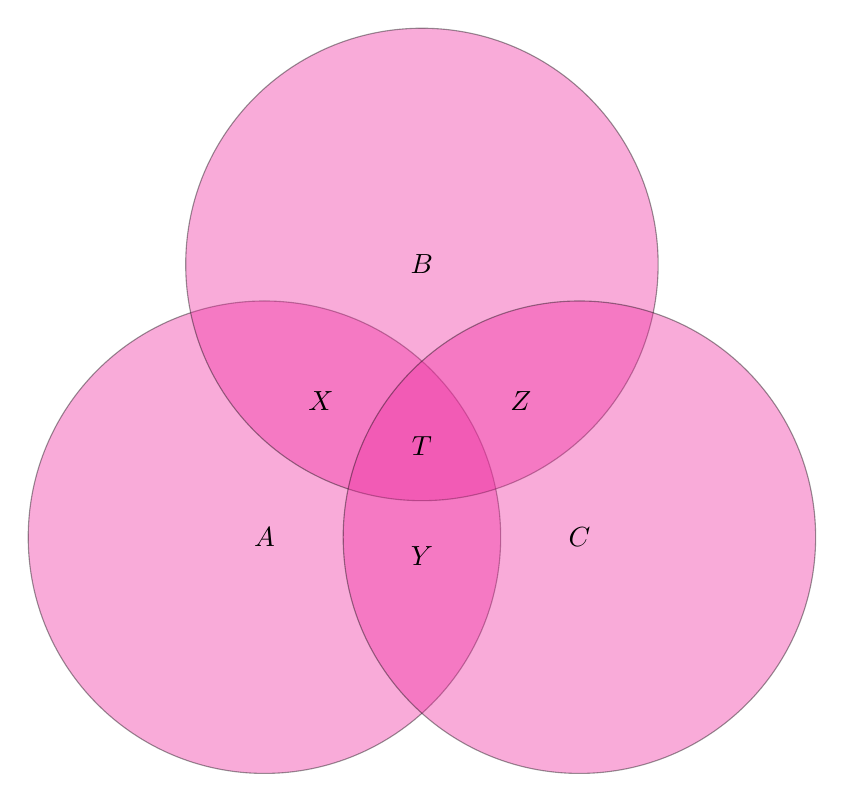
\begin{tikzpicture}[set/.style = {draw,
    circle,
    minimum size = 6cm,
    fill=Rhodamine,
    opacity = 0.4,
    text opacity = 1}]
 
\node (A) [set] {$A$};
\node (B) at (60:4cm) [set] {$B$};
\node (C) at (0:4cm) [set] {$C$};
 
\node at (barycentric cs:A=1,B=1) [left] {$X$};
\node at (barycentric cs:A=1,C=1) [below] {$Y$};
\node at (barycentric cs:B=1,C=1) [right] {$Z$};
\node at (barycentric cs:A=1,B=1,C=1) [] {$T$};
 
\end{tikzpicture}
\end{center}

\textbf{Le problème :} Si on additionne simplement $|A| + |B| + |C|$, on compte certaines zones plusieurs fois :
\begin{itemize}
    \item Les intersections deux à deux ($X$, $Y$, $Z$) sont comptées \textbf{deux fois}
    \item L'intersection triple ($T$) est comptée \textbf{trois fois}
\end{itemize}

\textbf{La solution :} On corrige en soustrayant les intersections deux à deux, mais alors l'intersection triple est comptée :
\begin{itemize}
    \item $+3$ fois dans la somme initiale
    \item $-3$ fois dans la soustraction des intersections deux à deux (car elle appartient à chacune)
    \item Donc $0$ fois au total ! Il faut la rajouter.
\end{itemize}

D'où la formule : $|A \cup B \cup C| = |A| + |B| + |C| - |A \cap B| - |A \cap C| - |B \cap C| + |A \cap B \cap C|$
\end{intuitionbox}

\begin{theorembox}[Principe d'Inclusion-Exclusion généralisé]
Pour $n$ ensembles finis $A_1, A_2, \dots, A_n$, on a :
\begin{align*}
|A_1 \cup A_2 \cup \cdots \cup A_n| = & \sum_{i=1}^n |A_i| \\
& - \sum_{1 \leq i < j \leq n} |A_i \cap A_j| \\
& + \sum_{1 \leq i < j < k \leq n} |A_i \cap A_j \cap A_k| \\
& - \cdots \\
& + (-1)^{n+1} |A_1 \cap A_2 \cap \cdots \cap A_n|
\end{align*}
Ce qui s'écrit plus compactement :
$$ \left| \bigcup_{i=1}^n A_i \right| = \sum_{k=1}^n (-1)^{k+1} \sum_{1 \leq i_1 < i_2 < \cdots < i_k \leq n} |A_{i_1} \cap A_{i_2} \cap \cdots \cap A_{i_k}| $$
\end{theorembox}

\begin{intuitionbox}[Généralisation]
La logique reste la même que pour trois ensembles, mais l'argument clé est de prouver que chaque élément est compté \textbf{exactement une fois}, peu importe le nombre d'ensembles auxquels il appartient.

Supposons qu'un élément $x$ est membre d'exactement $k$ ensembles parmi les $n$ ensembles $A_1, \ldots, A_n$. Analysons combien de fois $x$ est compté dans la formule :
\begin{itemize}
    \item \textbf{Première somme ($\sum |A_i|$)} : $x$ est dans $k$ ensembles, donc il est ajouté $k$ fois. Le nombre de fois est $\binom{k}{1}$.
    
    \item \textbf{Deuxième somme ($-\sum |A_i \cap A_j|$)} : On soustrait $x$ pour chaque paire d'ensembles auxquels il appartient. Il y a $\binom{k}{2}$ telles paires.
    
    \item \textbf{Troisième somme ($+\sum |A_i \cap A_j \cap A_k|$)} : On ajoute de nouveau $x$ pour chaque triplet d'ensembles auxquels il appartient. Il y en a $\binom{k}{3}$.
    
    \item \textbf{Et ainsi de suite...}
\end{itemize}

Au total, l'élément $x$ est compté :
$$ \binom{k}{1} - \binom{k}{2} + \binom{k}{3} - \cdots + (-1)^{k-1}\binom{k}{k} \text{ fois.} $$

Pour voir que cette somme vaut exactement 1, rappelons une identité fondamentale issue du binôme de Newton :
$$ (1-1)^k = \sum_{j=0}^{k} (-1)^j \binom{k}{j} = \binom{k}{0} - \binom{k}{1} + \binom{k}{2} - \cdots + (-1)^k \binom{k}{k} = 0 $$

En réarrangeant cette équation, sachant que $\binom{k}{0}=1$ :
$$ \binom{k}{0} = \binom{k}{1} - \binom{k}{2} + \binom{k}{3} - \cdots - (-1)^{k}\binom{k}{k} $$
$$ 1 = \binom{k}{1} - \binom{k}{2} + \binom{k}{3} - \cdots + (-1)^{k-1}\binom{k}{k} $$

Cela prouve que n'importe quel élément, qu'il soit dans un seul ensemble ($k=1$) ou dans plusieurs ($k>1$), contribue précisément pour 1 au décompte final. Le principe d'inclusion-exclusion est donc une méthode infaillible pour corriger les comptages multiples de manière systématique.
\end{intuitionbox}


\begin{examplebox}[Application probabiliste]
On lance trois dés équilibrés. Quelle est la probabilité d'obtenir au moins un 6 ?

\vspace{0.3cm}
\noindent\textbf{Solution avec inclusion-exclusion :}

Soit $A$ = "le premier dé montre 6", $B$ = "le deuxième dé montre 6", $C$ = "le troisième dé montre 6".

On veut $P(A \cup B \cup C)$.

\begin{align*}
P(A \cup B \cup C) &= P(A) + P(B) + P(C) \\
&\quad - P(A \cap B) - P(A \cap C) - P(B \cap C) \\
&\quad + P(A \cap B \cap C) \\
&= \frac{1}{6} + \frac{1}{6} + \frac{1}{6} - \frac{1}{36} - \frac{1}{36} - \frac{1}{36} + \frac{1}{216} \\
&= \frac{3}{6} - \frac{3}{36} + \frac{1}{216} = \frac{1}{2} - \frac{1}{12} + \frac{1}{216} \\
&= \frac{108 - 18 + 1}{216} = \frac{91}{216} \approx 0.421
\end{align*}

\vspace{0.3cm}
\noindent\textbf{Vérification par la méthode complémentaire :}
La probabilité de n'obtenir aucun 6 est $\left(\frac{5}{6}\right)^3 = \frac{125}{216}$, donc la probabilité d'au moins un 6 est $1 - \frac{125}{216} = \frac{91}{216}$.
\end{examplebox}